\section{Introduction}
\label{sec:intro}

The success of computer vision deep learning models relies heavily on the large amounts of data available for training on the internet \cite{8237359}.
In the domain of remote sensing, however, labeled data is hard to obtain because labeling is a complicated task that requires expert knowledge and there is a much wider range of sensors compared to standard RGB cameras of everyday cameras. \cite{dofa}.
There are multiple ways to address this issue, such as using synthetic data or semi-supervised learning algorithms. Following the breakthroughs of LLMs and the concept of pretraining foundation models on a wide range of tasks, recent research has attempted to transfer this concept to the area of remote sensing computer vision \cite{bommasani2022opportunitiesrisksfoundationmodels}.

This report focuses on one foundational model called 'DOFA' \cite{dofa}
and evaluates it on a new downstream task for comparison with other foundation models. The used dataset is called BigEarthNet \cite{bigearthnet}
and we will be utilizing the Sentinel-1 data. We will provide results using different metrics for the multi-label classification of both the 19-class and 43-class variants.

We will analyze the meaningfulness of the features computed by the DOFA model by applying a UMAP transformation \cite{umap-paper}. Afterward, we will use the features as input data for training various classifiers on the classification task.


\begin{figure}[h]
	\centering
	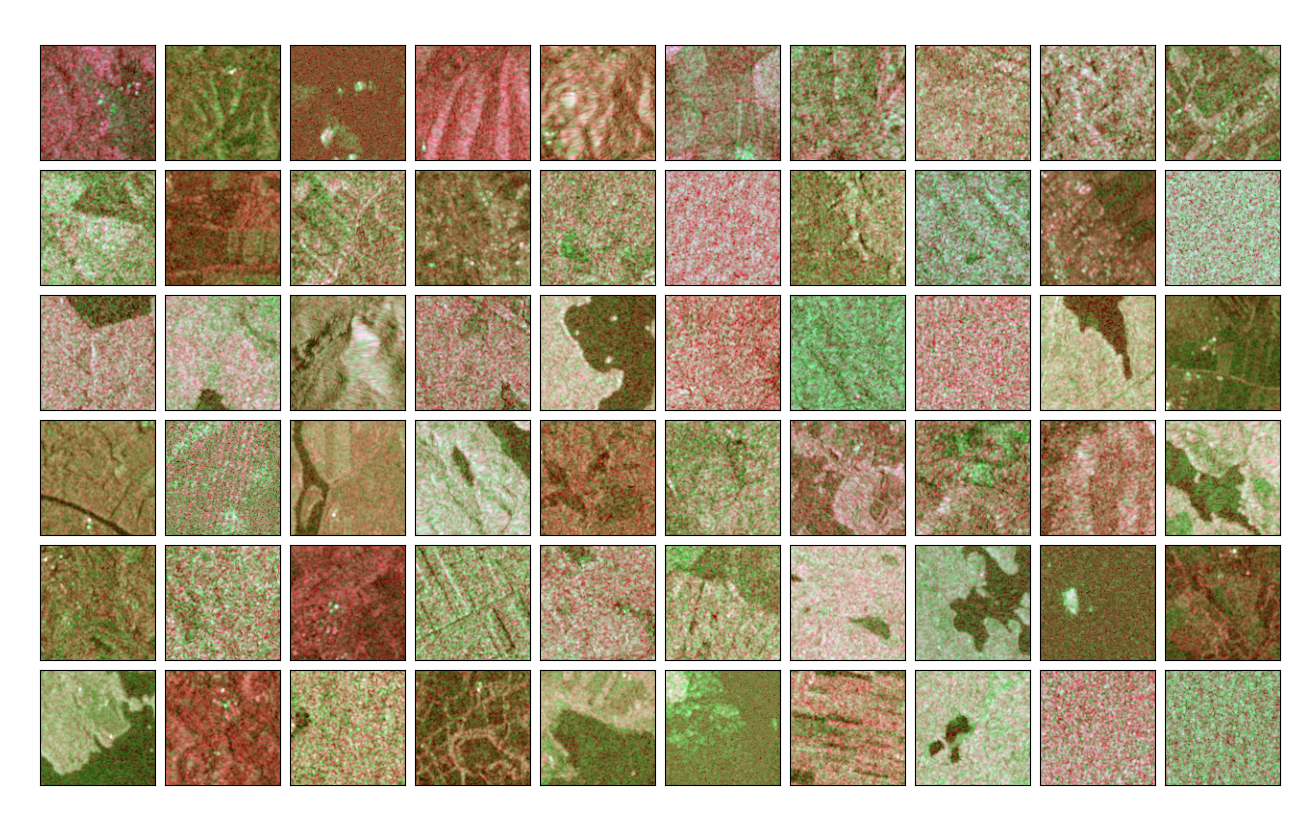
\includegraphics[width=\columnwidth]{images/example-images.png}
	\caption{False color visualization of some images from Sentinel-I satellites as part of the BigEarthNet dataset \cite{bigearthnet}}
	\label{fig:example-image}
\end{figure}